\documentclass[12pt,a4paper]{article}
\usepackage{azzam}
\usepackage{tikz}
\usepackage{float}
\usepackage{graphicx}

\begin{document}
\title{Kumpulan Soal OSN SMA 2002--2025 (Berdasarkan Topik)}
\begin{center}
    \Large \textbf{Kumpulan Soal Geometri OSN tingkat Nasional Matematika SMA 2002--2025}
\end{center}
\section{Geometri}

\subsection{G3. Teorema Pythagoras dan Perbandingan Trigonometri}
\begin{enumerate}

% osn sma 2006 nomor 3 esai
% Geometri: G3. Teorema Pythagoras dan Perbandingan Trigonometri
% Answer: Terbukti
\item (OSN 2006) Misalkan $S$ adalah himpunan semua segitiga $ABC$ yang memenuhi sifat $\tan A$, $\tan B$ dan $\tan C$ adalah bilangan-bilangan asli. Buktikan bahwa semua segitiga anggota $S$ sebangun.

% osn sma 2016 nomor 4 esai
% Geometri: G3. Teorema Pythagoras dan Perbandingan Trigonometri
% Answer: -
\item (OSN 2016) Misalkan dalam segitiga $ABC$ berlaku bahwa
$$\frac{\cos A}{20}+\frac{\cos B}{21}+\frac{\cos C}{29}=\frac{29}{420}$$
Buktikan bahwa segitiga $ABC$ merupakan segitiga siku-siku.

\end{enumerate}

\subsection{G4. Garis-Garis Istimewa Segitiga}
\begin{enumerate}

% osn sma 2006 nomor 5 esai
% Geometri: G4. Garis-Garis Istimewa Segitiga
% Answer: Terbukti
\item (OSN 2006) Pada segitiga $ABC$, $M$ adalah titik tengah $BC$ dan $G$ adalah titik berat segitiga $ABC$. Sebuah garis $l$ melalui $G$ memotong ruas garis $AB$ di $P$ dan ruas garis $AC$ di $Q$, dimana $P \ne B$ dan $Q \ne C$. Jika $[XYZ]$ menyatakan luas segitiga $XYZ$, tunjukkan bahwa
$$\frac{[BGM]}{[PAG]}+\frac{[CMG]}{[QGA]}=\frac{3}{2}$$

% osn sma 2007 nomor 1 esai
% Geometri: G4. Garis-Garis Istimewa Segitiga
% Answer: Terbukti
\item (OSN 2007) Misalkan $ABC$ segitiga dengan $\angle ABC=\angle ACB=70^{\circ}$. Misalkan titik $D$ pada sisi $BC$ sehingga $AD$ garis tinggi, titik $E$ pada sisi $AB$ sehingga $\angle ACE=10^{\circ}$, dan titik $F$ adalah perpotongan $AD$ dan $CE$. Buktikan bahwa $CF=BC.$

% osn sma 2009 nomor 3 esai
% Geometri: G4. Garis-Garis Istimewa Segitiga
% Answer: Terbukti
\item (OSN 2009) Pada segitiga $ABC$, titik-titik $D, E$ dan $F$ berturut-turut terletak pada segmen $BC, CA$ dan $AB$. Nyatakan $P$ sebagai titik perpotongan $AD$ dan $EF$. Tunjukkan bahwa
$$\frac{AF}{AB} \cdot \frac{DC}{BC} + \frac{AE}{AC} \cdot \frac{DB}{BC} = \frac{AP}{AD}$$

% osn sma 2009 nomor 8 esai
% Geometri: G4. Garis-Garis Istimewa Segitiga
% Answer: Terbukti
\item (OSN 2009) Diberikan segitiga $ABC$ lancip. Lingkaran dalam segitiga $ABC$ menyinggung $BC, CA,$ dan $AB$ berturut-turut di $D, E,$ dan $F$. Garis bagi sudut $A$ memotong $DE$ dan $DF$ berturut-turut di $K$ dan $L$. Misalkan $AA_{1}$ adalah garis tinggi dan $M$ titik tengah $BC$.
\begin{enumerate}
    \item Buktikan bahwa $BK$ dan $CL$ tegak lurus garis bagi sudut $BAC$.
    \item Tunjukkan bahwa $A_{1}KML$ adalah segiempat talibusur.
\end{enumerate}

\end{enumerate}

\subsection{G5. Lingkaran}
\begin{enumerate}

% osn sma 2004 nomor 4 esai
% Geometri: G5. Lingkaran
% Answer: Terbukti
\item (OSN 2004) Lingkaran yang berbeda bentuk disusun sebagai berikut:

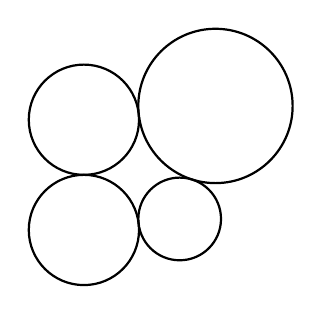
\begin{tikzpicture}[scale=0.35]
  \draw[thick] (0,2) circle (2);
  \draw[thick] (0,-2) circle (2);
  \draw[thick] (4.774,2.5) circle (2.8);
  \draw[thick] (3.475,-1.6) circle (1.5);
\end{tikzpicture}

Buktikan bahwa ada lingkaran yang melewati keempat titik singgung keempat lingkaran.

% osn sma 2004 nomor 7 esai
% Geometri: G5. Lingkaran
% Answer: Terbukti
\item (OSN 2004) Buktikan bahwa suatu segitiga $ABC$ siku-siku di $C$ dengan $a$ menyatakan sisi di hadapan sudut $A$, $b$ menyatakan sisi di hadapan sudut $B$, $c$ menyatakan sisi di hadapan sudut $C$ memiliki diameter lingkaran dalam $=a+b-c.$

% osn sma 2008 nomor 7 esai
% Geometri: G5. Lingkaran
% Answer: Terbukti
\item (OSN 2008) Diberikan segitiga $ABC$ dengan panjang sisi-sisinya $a, b,$ dan $c$. Garis-garis singgung lingkaran dalam segitiga $ABC$ yang sejajar dengan sisi-sisi segitiga $ABC$ membentuk tiga segitiga kecil. Pada masing-masing segitiga kecil dibuat lingkaran dalam. Buktikan bahwa jumlah luas dari lingkaran dalam segitiga $ABC$ dan ketiga lingkaran dalam segitiga kecil adalah
$$\frac{\pi(a^{2}+b^{2}+c^{2})(b+c-a)(c+a-b)(a+b-c)}{(a+b+c)^{3}}$$

% osn sma 2011 nomor 8 esai
% Geometri: G5. Lingkaran
% Answer: -
\item (OSN 2011) Diberikan segitiga sebarang $ABC$ dan misalkan lingkaran dalam segitiga $ABC$ menyinggung sisi $BC$, $CA$, dan $AB$ berturut-turut di titik $D$, $E$, dan $F$. Misalkan $K$ dan $L$ berturut-turut titik pada sisi $CA$ dan $AB$ sedemikian sehingga $\angle EDK=\angle ADE$ dan $\angle FDL=\angle ADF.$ Buktikan bahwa lingkaran luar segitiga $AKL$ menyinggung lingkaran dalam segitiga $ABC$.

% osn sma 2015 nomor 6 esai
% Geometri: G5. Lingkaran
% Answer: -
\item (OSN 2015) Diberikan segitiga lancip $ABC$ dengan titik pusat lingkaran luar $O$. Garis $AO$ memotong lingkaran luar segitiga $ABC$ lagi di titik $D$. Misalkan $P$ titik pada sisi $BC$. Garis melalui $P$ tegak lurus $AP$ memotong garis $DB$ dan $DC$ berturut-turut di $E$ dan $F$. Garis melalui $D$ tegak lurus $BC$ memotong $EF$ di titik $Q$. Buktikan bahwa $EQ=QG$ jika dan hanya jika $BP=CP$.

% osn sma 2020 nomor 1 esai
% Geometri: G5. Lingkaran
% Answer: -
\item (OSN 2020) Diberikan segitiga lancip $ABC$ dan titik $D$ pada segmen $BC$. Lingkaran $c_1$ adalah lingkaran yang melalui $A$, $D$, dan memiliki titik pusat pada garis $AC$, sedangkan lingkaran $c_2$ adalah lingkaran yang melalui $A$, $D$, dan memiliki titik pusat pada garis $AB$. Misalkan $P \neq A$ adalah titik potong lingkaran $c_1$ dengan $AB$ dan $Q \neq A$ adalah titik potong lingkaran $c_2$ dengan $AC$. Buktikan bahwa $AD$ garis bagi $\angle PDQ$.

% osn sma 2021 nomor 7 esai
% Geometri: G5. Lingkaran
% Answer: -
\item (OSN 2021) Diberikan segitiga $ABC$ dengan lingkaran luarnya $l$. Titik $M$ berada di dalam segitiga $ABC$ sehingga $AM$ garis bagi $\angle BAC$. Lingkaran dengan pusat $M$ dan jari-jari $MB$ memotong $l$ dan $BC$ berturut-turut di $D$ dan $E$ ($B \neq D$ dan $B \neq E$). Misalkan $P$ titik tengah busur $BC$ di $l$ yang tidak mengandung $A$. Buktikan $AP$ garis bagi $\angle DPE$ jika dan hanya jika $\angle B = 90^\circ$.

% osn sma 2022 nomor 6 esai
% Geometri: G5. Lingkaran
% Answer: -
\item (OSN 2022) Pada segitiga $ABC$, titik $D$ and $E$ berada pada sisi $AB$ and $AC$ berturut-turut sehingga $DE$ sejajar $BC$. Diketahui terdapat titik $P$ pada interior segiempat $BDEC$ sehingga
$$\angle BPD = \angle CPE = 90^\circ.$$
Buktikan bahwa garis $AP$ melalui titik pusat lingkaran luar dari segitiga-segitiga $EPD$ dan $BPC$.

% osn sma 2023 nomor 1 esai
% Geometri: G5. Lingkaran
% Answer: -
\item (OSN 2023) Diberikan segitiga lancip $ABC$ dengan sisi terpanjang $BC$. Titik $D, E$ berturut-turut pada $AC, AB$ sehingga $BA = BD$ dan $CA = CE$. Titik $A'$ merupakan pencerminan $A$ terhadap garis $BC$. Buktikan bahwa lingkaran luar segitiga $ABC$ dan $A'DE$ mempunyai panjang jari-jari yang sama.

% osn sma 2023 nomor 7 esai
% Geometri: G5. Lingkaran
% Answer: -
\item (OSN 2023) Diberikan segitiga $ABC$ dengan $\angle ACB = 90^\circ$. Misalkan $\omega$ lingkaran luar $ABC$. Garis singgung terhadap $\omega$ di titik $B$ dan $C$ bertemu di $P$. Misalkan $M$ titik tengah $P B$. Garis $CM$ memotong $\omega$ di $N$ dan garis $P N$ memotong $AB$ di $E$. Titik $D$ pada $CM$ sehingga $ED \parallel BM$. Buktikan bahwa lingkaran luar $CDE$ menyinggung $\omega$.

% osn sma 2025 nomor 8 esai
% Geometri: G5. Lingkaran
% Answer: Terbukti
\item (OSN 2025) Diberikan segitiga $ABC$ dengan sisi $BC$ lebih panjang dari sisi $CA$ dan $M$ adalah titik tengah sisi $AB$. Lingkaran dalam segitiga $ABC$ menyinggung sisi-sisi $BC, CA, AB$ berturut-turut di titik-titik $D, E, F$. Misalkan $G$ adalah titik potong garis $DE$ dan garis $AB$, $O$ adalah titik pusat lingkaran luar segitiga $FCG$, dan garis $OA$ memotong lingkaran luar segitiga $FOG$ di titik $H \ (H \ne O)$. Jika $\angle OCB = 90^{\circ}$, buktikan bahwa $MH$ menyinggung lingkaran luar segitiga $FOG$.

\end{enumerate}

\subsection{G6. Segiempat dan Poligon}
\begin{enumerate}

% osn sma 2002 nomor 7 esai
% Geometri: G6. Segiempat dan Poligon
% Answer: Terbukti
\item (OSN 2002) Misalkan $ABCD$ sebuah belah ketupat dengan $\angle A=60^{\circ}$ dan $P$ adalah titik potong kedua diagonal $AC$ dan $BD$. Misalkan $Q, R$ dan $S$ tiga titik pada (keliling) belah ketupat. Jika $PQRS$ juga membentuk belah ketupat, tunjukkan bahwa tepat satu di antara $Q, R, S$ berimpit dengan titik sudut belah ketupat $ABCD$.

% osn sma 2003 nomor 2 esai
% Geometri: G6. Segiempat dan Poligon
% Answer: Terbukti
\item (OSN 2003) Diberikan sebuah segiempat $ABCD$ sebarang. Misalkan $P, Q, R, S$ berturut-turut adalah titik-titik tengah $AB, BC, CD, DA$. Misalkan pula $PR$ dan $QS$ berpotongan di $O$. Buktikan bahwa $PO=OR$ dan $QO=OS$.

% osn sma 2005 nomor 7 esai
% Geometri: G6. Segiempat dan Poligon
% Answer: Terbukti
\item (OSN 2005) Misalkan $ABCD$ sebuah segiempat konveks. Persegi $AB_{1}A_{2}B$ dibuat sehingga kedua titik $A_{2}, B_{1}$ terletak di luar segiempat $ABCD$. Dengan cara serupa diperoleh persegi-persegi $BC_{1}B_{2}C$, $CD_{1}C_{2}D$ dan $DA_{1}D_{2}A$. Misalkan $K$ adalah titik potong $AA_{2}$ dengan $BB_{1}$, $L$ adalah titik potong $BB_{2}$ dengan $CC_{1}$, $M$ adalah titik potong $CC_{2}$ dengan $DD_{1}$, dan $N$ adalah titik potong $DD_{2}$ dengan $AA_{1}$. Buktikan bahwa $KM$ tegak lurus $LN$.

% osn sma 2013 nomor 7 esai
% Geometri: G6. Segiempat dan Poligon
% Answer: -
\item (OSN 2013) Diberikan jajar genjang $ABCD$. Pada sisi luar jajar genjang, dikonstruksi persegi-persegi $ABC_{1}D_{1}$, $BCD_{2}A_{2}$, $CDA_{3}B_{3}$ dan $DAB_{4}C_{4}$. Pada sisi-sisi luar $B_{4}D_{1}$, $C_{1}A_{2}$, $D_{2}B_{3}$, dan $A_{3}C_{4}$ dari segitiga-segitiga $AB_{4}D_{1}$, $BC_{1}A_{2}$, $CD_{2}B_{3}$, dan $DA_{3}C_{4}$, konstruksi persegi-persegi lagi dengan pusat berturut-turut $O_{A}$, $O_{B}$, $O_{C}$ dan $O_{D}$. Buktikan bahwa $AO_{A}=BO_{B}=CO_{C}=DO_{D}$.

% osn sma 2014 nomor 3 esai
% Geometri: G6. Segiempat dan Poligon
% Answer: -
\item (OSN 2014) Diberikan trapesium $ABCD$ dengan $AB$ sejajar $CD$ dan $AB<CD$. Misalkan diagonal $AC$ dan $BD$ bertemu di $E$ dan misalkan garis $AD$ dan $BC$ bertemu di titik $F$. Bangun jajar genjang $AEDK$ dan $BECL$. Buktikan bahwa garis $EF$ melalui titik tengah segmen $KL$.

% osn sma 2017 nomor 1 esai
% Geometri: G6. Segiempat dan Poligon
% Answer: -
\item (OSN 2017) Misalkan titik sudut $A$ dari jajar genjang $ABCD$, dibuat suatu garis $g$. Buktikan bahwa jarak dari $C$ ke garis $g$ adalah jumlah atau selisih jarak dari $B$ dan $D$ ke $g$.

% osn sma 2017 nomor 7 esai
% Geometri: G6. Segiempat dan Poligon
% Answer: -
\item (OSN 2017) Diberikan jajar genjang $ABCD$. Titik $E$ dan titik $F$ dipilih berturut-turut pada sisi $BC$ dan $CD$ sedemikian rupa sehingga segitiga $ABE$ dan segitiga $BCF$ mempunyai luas yang sama. Diagonal $BD$ memotong $AE$ and $AF$ berturut-turut di $M$ dan $N$. Buktikan terdapat segitiga yang panjang sisi-sisinya sama dengan $BM, MN,$ dan $ND$.

% osn semifinal sma 2026 nomor 2 esai
% Geometri: G6. Segiempat dan Poligon
% Answer: 50 derajat
\item (OSN Semifinal 2026) Diberikan segiempat konveks $ABCD$ dengan
$$\angle ABC = 140^{\circ} \text{ dan } \angle ACD = 110^{\circ}.$$
Misalkan diagonal $AC$ dan $BD$ berpotongan di titik $E$. Diketahui bahwa titik pusat lingkaran luar segitiga $CED$ terletak pada garis $AD$ dan titik pusat lingkaran luar segitiga $BEC$ terletak pada perpanjangan garis $AB$.

Tentukan nilai $\angle BAD$.

\end{enumerate}

\subsection{G10. Konkurensi}
\begin{enumerate}

% osn sma 2008 nomor 1 esai
% Geometri: G10. Konkurensi
% Answer: Terbukti
\item (OSN 2008) Diberikan segitiga $ABC$. Titik-titik $D, E,$ dan $F$ di luar segitiga $ABC$ sedemikian sehingga segitiga $ABD$, segitiga $BCE$, dan segitiga $CAF$ adalah segitiga sama sisi. Buktikan bahwa ketiga lingkaran luar segitiga tersebut berpotongan di satu titik.

% osn sma 2010 nomor 2 esai
% Geometri: G10. Konkurensi
% Answer: -
\item (OSN 2010) Diberikan segitiga lancip $ABC$ dengan $AB>BC$ dan titik pusat lingkaran luar $O$. Garis tinggi segitiga $ABC$ dari $C$ memotong $AB$ dan lingkaran luar segitiga $ABC$ lagi berturut-turut di titik $D$ dan $E$. Garis melalui $O$ sejajar $AB$ memotong garis $AC$ di titik $F$. Buktikan bahwa garis $CO$, garis melalui $F$ tegak lurus $AC$, dan garis melalui $E$ sejajar $DO$ bertemu di satu titik.

% osn sma 2013 nomor 2 esai
% Geometri: G10. Konkurensi
% Answer: -
\item (OSN 2013) Diberikan segitiga lancip $ABC$ dengan lingkaran luar $\omega$. Garis bagi $\angle BAC$ memotong $\omega$ di titik $M$. Misalkan $P$ suatu titik pada garis $AM$ dengan $P$ di dalam segitiga $ABC$. Garis melalui $P$ yang sejajar $AB$ dan garis melalui $P$ yang sejajar $AC$ memotong sisi $BC$ berturut-turut di titik $E$ dan $F$. Garis $ME$ dan $MF$ memotong $\omega$ lagi berturut-turut di titik $K$ dan $L$. Buktikan bahwa garis-garis $AM$, $BL$ dan $CK$ konkuren.

% osn sma 2022 nomor 3 esai
% Geometri: G10. Konkurensi
% Answer: -
\item (OSN 2022) Diberikan persegi panjang $ABCD$. Titik $E, F$ terletak pada diagonal $AC$ sehingga $F$ di antara $A, E$ dan $E$ terletak di antara $C, F$. Lingkaran luar segitiga $BEF$ memotong $AB$ dan $BC$ pada $G, H$ dan lingkaran luar segitiga $DEF$ memotong $AD$ dan $CD$ pada $I, J$. Buktikan bahwa $GJ, IH,$ dan $AC$ berpotongan di satu titik.

\end{enumerate}

\subsection{G11. Kolinearitas dan Kesegarisan}
\begin{enumerate}

% osn sma 2007 nomor 7 esai
% Geometri: G11. Kolinearitas dan Kesegarisan
% Answer: Terbukti
\item (OSN 2007) Titik-titik $A, B, C, D$ terletak pada lingkaran $S$ demikian rupa, sehingga $AB$ merupakan garis tengah $S$, tetapi $CD$ bukan garis tengah $S$. Diketahui pula bahwa $C$ dan $D$ berada pada sisi yang berbeda terhadap $AB$. Garis singgung terhadap $S$ di $C$ dan $D$ berpotongan di titik $P$. Titik-titik $Q$ dan $R$ berturut-turut adalah perpotongan garis $AC$ dengan garis $BD$ dan garis $AD$ dengan garis $BC$.
\begin{enumerate}
    \item Buktikan bahwa $P,Q$ dan $R$ segaris.
    \item Buktikan bahwa garis $QR$ tegak lurus terhadap garis $AB$.
\end{enumerate}

% osn sma 2012 nomor 8 esai
% Geometri: G11. Kolinearitas dan Kesegarisan
% Answer: -
\item (OSN 2012) Diberikan segitiga sebarang $ABC$ dan garis bagi $\angle BAC$ memotong sisi $BC$ dan lingkaran luar segitiga $ABC$ berturut-turut di titik $D$ dan $E$. Misalkan $M$ dan $N$ berturut-turut titik tengah $BD$ dan $CE$. Lingkaran luar segitiga $ABD$ memotong $AN$ di titik $Q$. Lingkaran yang melalui $A$ dan menyinggung $BC$ di $D$ memotong garis $AM$ dan sisi $AC$ berturut-turut di titik $P$ dan $R$. Tunjukkan bahwa empat titik $B, P, Q, R$ terletak pada satu garis.

% osn sma 2015 nomor 3 esai
% Geometri: G11. Kolinearitas dan Kesegarisan
% Answer: -
\item (OSN 2015) Diberikan segitiga lancip $ABC$. Lingkaran $\Gamma_{B}$ adalah lingkaran yang melewati $AB$ dan menyinggung $AC$ pada $A$ dan berpusat di $O_{B}$. Definisikan serupa untuk $\Gamma_{C}$ dan $O_{C}$. Misalkan garis tinggi segitiga $ABC$ dari $B$ dan $C$ memotong lingkaran luar segitiga $ABC$ pada $X$ dan $Y$. Buktikan $A$, titik tengah $XY$, dan titik tengah $O_{B}O_{C}$ segaris.

% osn sma 2018 nomor 8 esai
% Geometri: G11. Kolinearitas dan Kesegarisan
% Answer: -
\item (OSN 2018) Misalkan $I$ dan $O$ masing-masing menyatakan titik pusat lingkaran dalam dan lingkaran luar dari segitiga $ABC$. Lingkaran singgung luar $\omega_{A}$ dari segitiga $ABC$ menyinggung sisi $BC$ di $N$ serta menyinggung perpanjangan sisi $AB$ dan $AC$ masing-masing di $K$ dan $M$. Jika titik tengah dari ruas garis $KM$ berada pada lingkaran luar segitiga $ABC$, buktikan bahwa $O, I,$ dan $N$ segaris.

% osn sma 2024 nomor 3 esai
% Geometri: G11. Kolinearitas dan Kesegarisan
% Answer: -
\item (OSN 2024) Diberikan segitiga $ABC$ yang lingkaran luarnya berpusat di $O$ dan ketiga garis tingginya berpotongan di $H$. Garis $AH$ dan garis $BH$ memotong lingkaran luar segitiga $ABC$ sekali lagi berturut-turut di titik $D$ dan $E$. Misalkan $A'$ dan $B'$ berturut-turut menyatakan titik pusat lingkaran luar segitiga $AHE$ dan lingkaran luar segitiga $BHD$. Jika $A', B', O,$ dan $H$ tidak segaris, buktikan $OH$ melalui titik tengah ruas garis $A'B'$.

\end{enumerate}

\subsection{G12. Segiempat Konsiklis}
\begin{enumerate}

% osn sma 2016 nomor 1 esai
% Geometri: G12. Segiempat Konsiklis
% Answer: -
\item (OSN 2016) Diberikan segiempat talibusur $ABCD$ dengan kedua diagonalnya saling tegak lurus dan berpotongan di titik $O$. Garis tegak lurus dari $O$ pada $AB$, memotong $AB$ di $E$. Garis tegak lurus dari $O$ pada $BC$, memotong $BC$ di $F$. Garis tegak lurus dari $O$ pada $CD$, memotong $CD$ di $G$. Garis tegak lurus $O$ pada $DA$, memotong $DA$ di $H$.
\begin{enumerate}
    \item[(a)] Buktikan bahwa $\angle EFG+\angle GHE=180^{\circ}$.
    \item[(b)] Buktikan bahwa $OE$ merupakan garis bagi sudut $FEH$.
\end{enumerate}

% osn sma 2018 nomor 2 esai
% Geometri: G12. Segiempat Konsiklis
% Answer: -
\item (OSN 2018) Misalkan $\Gamma_{1}$ dan $\Gamma_{2}$ dua lingkaran yang bersinggungan di titik $A$ dengan $\Gamma_{2}$ di dalam $\Gamma_{1}$. Misalkan $B$ titik pada $\Gamma_{2}$ dan garis $AB$ memotong $\Gamma_{1}$ di titik $C$. Misalkan $D$ titik pada $\Gamma_{1}$ dan $P$ sebarang titik pada garis $CD$ (boleh pada perpanjangan segmen $CD$). Garis $BP$ memotong $\Gamma_{2}$ di titik $Q$. Tunjukkan bahwa $A, D, P, Q$ terletak pada satu lingkaran.

% osn sma 2020 nomor 6 esai
% Geometri: G12. Segiempat Konsiklis
% Answer: -
\item (OSN 2020) Diberikan segiempat talibusur $ABCD$. Misalkan $X$ titik pada sisi $BC$ ($X \neq C$) sehingga garis $AX$ tegak lurus dengan garis bagi $\angle CBD$, dan $Y$ titik pada sisi $AD$ ($Y \neq D$) sehingga garis $BY$ tegak lurus dengan garis bagi $\angle CAD$. Buktikan bahwa $XY$ sejajar dengan $CD$.

% osn sma 2021 nomor 2 esai
% Geometri: G12. Segiempat Konsiklis
% Answer: -
\item (OSN 2021) Diberikan segitiga lancip $ABC$. Titik $D$ dan $E$ berturut-turut merupakan titik tengah segmen $AB$ dan $AC$. Misalkan $L_1$ dan $L_2$ berturut-turut lingkaran luar segitiga $ABC$ dan $ADE$. Garis $CD$ memotong lingkaran $L_1$ dan $L_2$ pada $M$ ($M \neq C$) dan $N$ ($N \neq D$). Jika $DM = DN$, buktikan bahwa $ABC$ segitiga sama kaki.

% osn semifinal sma 2025 nomor 4 esai
% Geometri: G12. Segiempat Konsiklis
% Answer: -
\item (OSN Semifinal 2025) Diberikan segitiga lancip $ABC$. Titik $D$ and $E$ berturut-turut terletak pada $AB$ and $AC$ sehingga $B, C, E, D$ terletak pada suatu lingkaran, katakan $\Gamma$. Misalkan $F$ titik pada lingkaran $\Gamma$ sehingga $EF \parallel AB$ dan $G\ne F$ titik pada lingkaran $\Gamma$ sehingga $A, G, F$ segaris, serta $H$ merupakan perpotongan garis $AB$ dan $CG$. Jika $I$ titik tengah ruas garis $BD$ dan $J$ titik pada sisi $AB$ sehingga $H$ titik tengah $AJ$, tununjukkan bahwa $CEJI$ merupakan segiempat talibusur.

\end{enumerate}

\subsection{G13. Ketaksamaan Geometri}
\begin{enumerate}

% osn sma 2005 nomor 4 esai
% Geometri: G13. Ketaksamaan Geometri
% Answer: Terbukti
\item (OSN 2005) Misalkan $M$ suatu titik di dalam segitiga $ABC$ sedemikian rupa hingga $\angle AMC = 90^{\circ}$, $\angle AMB = 150^{\circ}$ dan $\angle BMC = 120^{\circ}$. Titik pusat lingkaran luar dari segitiga-segitiga $AMC$, $AMB$ dan $BMC$ berturut-turut adalah $P, Q$ dan $R$. Buktikan bahwa luas segitiga $PQR$ lebih besar dari luas segitiga $ABC$.

% osn sma 2011 nomor 3 esai
% Geometri: G13. Ketaksamaan Geometri
% Answer: -
\item (OSN 2011) Diberikan sebarang segitiga lancip $ABC$. Misalkan $l_{a}$ adalah garis yang melalui $A$ dan tegak lurus $AB$, $l_{b}$ adalah garis yang melalui $B$ dan tegak lurus $BC$, $l_{c}$ adalah garis yang melalui $C$ dan tegak lurus $CA$. Misalkan garis $l_{b}$ dan $l_{c}$ berpotongan di titik $D$, garis $l_{c}$ dan $l_{a}$ berpotongan di titik $E$ dan terakhir, garis $l_{a}$ dan $l_{b}$ berpotongan di titik $F$. Buktikan bahwa luas segitiga $DEF$ paling sedikit tiga kali luas segitiga $ABC$.

% osn sma 2024 nomor 6 esai
% Geometri: G13. Ketaksamaan Geometri
% Answer: -
\item (OSN 2024) Diberikan $A_1, A_2, \dots, A_n$, suatu segi-$n$ dengan $n \ge 3$ dan $\angle A_j \le 180^\circ$ untuk setiap $j$. Untuk setiap $i \le n$, misalkan $\alpha_i$ adalah nilai terkecil yang mungkin dari $\angle A_i A_j A_{i+1}$ dengan $j$ berbeda dari $i$ dan $i + 1$. (Di sini kita definisikan $A_{n+1} = A_1$). Buktikan bahwa
$$\alpha_1 + \alpha_2 + \dots + \alpha_n \le 180^\circ.$$
Tentukan seluruh kasus dimana kesamaan terjadi.

\end{enumerate}

\subsection{G14. Geometri Kombinatorial}
\begin{enumerate}

% osn sma 2016 nomor 6 esai
% Geometri: G14. Geometri Kombinatorial
% Answer: -
\item (OSN 2016) Diberikan segiempat $ABCD$ yang kedua diagonalnya tidak saling tegak lurus. Suatu persegi dikatakan fantastik jika masing-masing garis sisi persegi tersebut memuat tepat satu titik yang berbeda di antara $A, B, C, D$. Buktikan bahwa sebarang segiempat $ABCD$ memiliki paling sedikit 6 persegi fantastik.

\textit{Catatan: Garis sisi adalah sisi dan perpanjangannya.}

\end{enumerate}

\subsection{G15. Kesamaan Panjang dan Rasio}
\begin{enumerate}

% osn sma 2002 nomor 4 esai
% Geometri: G15. Kesamaan Panjang dan Rasio
% Answer: Terbukti
\item (OSN 2002) Diberikan segitiga $ABC$ dengan $AC>BC$. Pada lingkaran luar segitiga $ABC$ terletak titik $D$ yang merupakan titik tengah busur $AB$ yang memuat titik $C$. Misalkan $E$ adalah titik pada $AC$ sehingga $DE$ tegak lurus pada $AC$.
Buktikan bahwa $AE=EC+CB$.

% osn sma 2010 nomor 8 esai
% Geometri: G15. Kesamaan Panjang dan Rasio
% Answer: -
\item (OSN 2010) Diberikan segitiga lancip $ABC$ dengan titik pusat lingkaran luar $O$ dan titik tinggi $H$. Misalkan $K$ sebarang titik di dalam segitiga $ABC$ yang tidak sama dengan $O$ maupun $H$. Titik $M$ dan $L$ terletak di luar segitiga $ABC$ sedemikian sehingga $AKCL$ dan $AKBM$ jajaran genjang. Terakhir, misalkan $BL$ dan $CM$ berpotongan di titik $N$ dan misalkan juga $J$ adalah titik tengah $HK$. Buktikan bahwa $KONJ$ jajaran genjang.

% osn sma 2012 nomor 3 esai
% Geometri: G15. Kesamaan Panjang dan Rasio
% Answer: -
\item (OSN 2012) Diberikan segitiga lancip $ABC$ dengan titik pusat lingkaran luar $O$ dan memenuhi $AB>AC$. Garis $BO$ dan $CO$ memotong garis bagi $\angle BAC$ berturut-turut di titik $P$ dan $Q$. Selanjutnya, garis $BQ$ dan $CP$ berpotongan di titik $R$. Buktikan bahwa $AR$ tegak lurus $BC$.

% osn sma 2014 nomor 6 esai
% Geometri: G15. Kesamaan Panjang dan Rasio
% Answer: -
\item (OSN 2014) Diberikan segitiga $ABC$ dengan $AD$ sebagai garis bagi dalam $\angle BAC$. Misalkan titik $M$ dan $N$ berturut-turut pada $AB$ dan $AC$ sehingga $\angle MDA=\angle ABC$ dan $\angle NDA=\angle ACB$. Jika $P$ merupakan titik potong dari garis $AD$ dan garis $MN$, buktikan bahwa $AD^{3}=AB\cdot AC\cdot AP.$

% osn sma 2019 nomor 3 esai
% Geometri: G15. Kesamaan Panjang dan Rasio
% Answer: -
\item (OSN 2019) Diberikan sebuah persegi panjang $ABCD$ dengan $AD > AB$. Misalkan titik $E$ pada $AD$ sehingga $BE \perp AC$ dan $BE$ memotong $AC$ di $M$. Lingkaran luar segitiga $BEA$ memotong $AC$ dan $BC$ berturut-turut di $N$ dan $F$. Lingkaran luar segitiga $DEN$ memotong $CD$ di $G$. Misalkan $FG$ memotong $AB$ di $P$. Buktikan bahwa $PM = PN$.

% osn sma 2019 nomor 6 esai
% Geometri: G15. Kesamaan Panjang dan Rasio
% Answer: -
\item (OSN 2019) Diberikan sebuah lingkaran yang berpusat di $O$. Diketahui suatu titik $A$ tidak terletak pada keliling lingkaran dan $B$ adalah refleksi $A$ terhadap $O$. Titik $P$ terletak sembarang pada keliling lingkaran. Garis tegak lurus $AP$ melalui $P$ memotong lingkaran tersebut di $Q$. Buktikan bahwa $AP \times BQ$ konstan di mana pun letak titik $P$.

% osn sma 2025 nomor 2 esai
% Geometri: G15. Kesamaan Panjang dan Rasio
% Answer: Terbukti
\item (OSN 2025) Diberikan segitiga lancip $ABC$ dengan titik pusat lingkaran luar $O$. Titik $D$ dan $E$ terletak pada lingkaran luar segitiga $ABC$ sehingga $AD$ tegak lurus $BC$ dan $BE$ tegak lurus $CA$. Ruas garis $CD$ memotong lingkaran berdiameter $DO$ di titik $P$, sedangkan ruas garis $CE$ memotong lingkaran berdiameter $EO$ di titik $Q$. Buktikan bahwa $OP = OQ$.

\end{enumerate}

\end{document}